\documentclass[journal]{IEEEtran}
\usepackage{cite}
% *** GRAPHICS RELATED PACKAGES ***
%
\ifCLASSINFOpdf
  \usepackage[pdftex]{graphicx}
\fi
%
\usepackage[cmex10]{amsmath}


% *** ALIGNMENT PACKAGES ***
%
\usepackage{array}
\usepackage{fixltx2e}


\usepackage{stfloats}
% LaTeX2e). It also provides a command:
\fnbelowfloat

\usepackage{pgf}
\usepackage{tikz}
\usetikzlibrary{arrows,positioning}
\usepackage{url}
\usepackage{color}
\usepackage{graphicx}
\usepackage{xspace}
\newcommand*{\eg}{e.g.\@\xspace}
\newcommand*{\ie}{i.e.\@\xspace}

% correct bad hyphenation here
\hyphenation{op-tical net-works semi-conduc-tor}

\usepackage{color}
\newcommand{\vl}[1]{\textcolor{orange}{Vincent : #1}}
\newcommand{\gl}[1]{\textcolor{red}{Gr\'egoire : #1}}
\newcommand{\ja}[1]{\textcolor{magenta}{Joakim : #1}}
\newcommand{\ml}[1]{\textcolor{blue}{ Mathieu : #1}}



\begin{document}
%
% paper title
% can use linebreaks \\ within to get better formatting as desired
% Do not put math or special symbols in the title.
%\title{An evaluation framework for event detection using a morphological model of acoustic scenes}
\title{Acoustic Scene Classification: \\ Supervised and Unsupervised Approaches using the Scattering Transform}

\author{Vincent Lostanlen, Gr\'egoire Lafay, Joakim And\'en, and Mathieu Lagrange}


% make the title area
\maketitle

% As a general rule, do not put math, special symbols or citations
% in the abstract or keywords.
\begin{abstract}
This paper introduces a 
\end{abstract}

% Note that keywords are not normally used for peerreview paper.
\begin{IEEEkeywords}
Acoustic scene classification, segmentation.
\end{IEEEkeywords}






% For peer review papers, you can put extra information on the cover
% page as needed:
% \ifCLASSOPTIONpeerreview
% \begin{center} \bfseries EDICS Category: 3-BBND \end{center}
% \fi
%
% For peerreview papers, this IEEEtran command inserts a page break and
% creates the second title. It will be ignored for other modes.
\IEEEpeerreviewmaketitle

\section{Introduction}

\IEEEPARstart{O}{ver} the past decades, the amount of audio data recorded from our sonic environment has considerably grown. Recent research areas such as eco-acoustics \cite{ECOACOUSTICS2014, krause} start to consider massive deployment of acoustic sensors around the world in order to measure potential animal biodiversity modification over large temporal scales due to human activity or climate change \cite{NessSST13, stowell13a, stowell13b}. 

Also, some recent works demonstrate the interest of such approaches for the characterization of human acoustic pleasantness in urban areas \cite{lafay, lavandier} and the prediction of annoyance due to the traffic \cite{gloaguen}. We believe that those case study are of interest for the signal processing community as they have strong societal impacts and raises interesting research avenues. Unfortunately, those fields of research are still in infancy and consequently very few well built datasets are available for evaluation purposes. 

A closely related field of investigation that is relatively more mature is the classification of acoustic scenes whose aim is to predict labels by processing audio data. Despite its lower value, it has the advantage of being rooted by numerous works in cognitive psychology on categorization \cite{dubois} and been considered in the data processing field for a while, with availability of some well designed evaluation datasets. 

In this paper, we investigate the potential of a new unsupervised segmentation paradigm that allows us to 

This data has to be processed


Environment sound

describe in terms of high level attributes

be they cognitive ones such as pleasantness, or descriptive ones such as the type of environment where the 


%As part of the aforementioned research areas and applications, the emerging field of \emph{Acoustic Scene Analysis} (also called \emph{Sound Scene Analysis}) \cite{Stowell15} aims to develop approaches and systems for the automatic analysis of environmental sounds and soundscapes (originating both from urban or nature environments). While research methodologies in related fields such as Automatic Speech Recognition (ASR) \cite{Rabiner93} and Music Information Retrieval (MIR) \cite{Muller07} are now well established, research addressing Acoustic Scene Analysis remains relatively young. 

Whilst the range of applications are very large, so is the need

holistic / event based

skeleton of events on a bed of texture.

debate about the kind of process underlying perception

strong indication that the detection of specific events, named markers suffice to trigger class prediction

From a numerical data processing overview, the holistic scheme as a simplicity, but clearly face poor performance on realistic conditions \cite{lagrange:hal-01082501}.

If available, the complete description of the scene in terms of event occurences is powerful enough to reliably predict high level cognitive classes, \textit{i.e.} the presence of birds are strong pleasantness indicators and very likely to be heard in parks in urban areas.

\section{Previous work}

GL 1

ML 2

\subsection{Goal}

\subsection{Methods}

\subsection{Datasets}

defreville \cite{aucouturier2007bag}

\cite{lagrange:hal-01082501}

dcase2013 \cite{7100934} \cite{giannoulis2013database}

For each scene type, three different recordists (DG, DS,
EB) visited a wide variety of locations in Greater London over
a period of months (Summer and Autumn 2012), and in each
scene recorded a few minutes of audio. We ensured that no
systematic variations in the recordings covaried with scene
type: all recordings were made in moderate weather condi-
tions, and varying times of day and week, and each recordist
recorded each scene type.

Rouen \cite{rakotomamonjy2015histogram}

\url{https://sites.google.com/site/alainrakotomamonjy/home/audio-scene}

dCase2016 \cite{Mesaros2016_EUSIPCO}

advantages of dcase2013:

controled intra class diversity

despite its size, it is still challenging as state-of-the-art systems achieves 76 \% \cite{6701890} (winner of the 2013 challenge RQA+SVM). For the sake of comparison the HOG+SVM approach \cite{rakotomamonjy2015histogram} achieves 75 \% and 92 \% on the dcase2013 and the Rouen datasets respectively. On the latter, the state-of-the-art is currently 95 \% \cite{bisot2016acoustic}.

\section{Scattering representations}
Scattering transforms are translation-invariant representations of audio signals which cascade an auditory filterbank and a modulation filterbank, interspersed with complex modulus nonlinearities.
Depending upon the chosen architecture, the modulation filterbank may either be performed solely over the time variable or on both time and frequency.
In this section, we present both the temporal scattering transform and the time-frequency scattering transform.

\subsection{Invariance and stability in acoustic scene classification}
The notion of invariance to translation plays an essential role in auditory scene classification.
Indeed, the starting time of the recordings are chosen arbitrarily, and thus do not convey any information about the class.
To cancel this superfluous source of variability, signals must be mapped to a translation-invariant feature space prior to training the classifier.
From any set of descriptors -- \eg the time-frequency representation $\boldsymbol{x_1}(t,\gamma_1)$ of  a signal $\boldsymbol{x}(t)$ --
a translation-invariant representation up to time skills of duration $T$ can be simply obtained
by convolving $\boldsymbol{x_1}$ with a low-pass filter $\boldsymbol{\phi}(t)$ of cutoff frequency
set to $1/T$:
\begin{equation}
\mathbf{S_1}\boldsymbol{x}(t, \gamma_1) = (\boldsymbol{x_1} \ast \boldsymbol{\phi}) (t).
\end{equation}
As a downside, the transient information in $\boldsymbol{x_1}$ at finer scales than $T$ are lost by this low-pass filtering, hence a lack of discriminability in feature space.
To address this issue, the temporal scattering transform recovers this information by convolving $\boldsymbol{x_1}$ with wavelets whose center frequencies are above $1/T$, and subsequently applying complex modulus.

By resorting to wavelet modulus, as opposed to Fourier transform modulus, the resulting features are provably stable to small time warps,
in the sense of Lipschitz regularity with respect to diffeomorphisms \cite{Mallat2012}.
Besides invariance to translation, this stability property is crucial in signal classification, as it entails a guarantee of robustness to small variations in pitch, reverberation, and rhythmic organization of events, which make up an important part of the intra-class variability among natural sounds.

The scattering transform is defined mathematically as an infinite cascade of nonlinear layers, each consisting of a wavelet transform modulus operator.
In practice, to achieve invariance to translation up to $T = 186\,\mathrm{ms}$, \ie of the order of the minimal duration between non-overlapping acoustic events, two layers of scattering transform of the audio signal $\boldsymbol{x}(t)$ suffice.
The next subsection describes the operations involved in temporal scattering.

\subsection{Temporal scattering}
Let $\boldsymbol{\psi}(t)$ a complex-valued band-pass filter of
center frequency $\xi_1$ and bandwidth $\xi_1/Q_1$.
A filter bank of wavelets is built by dilating $\boldsymbol{\psi}(t)$
according to a geometric sequence of scales $2^{\gamma_1/Q_1}$.
The variable $\gamma_1$, akin to a log-frequency, takes integer values between $0$ and $(J_1 \times Q_1 - 1)$.
In the sequel, we set $\xi_1$ to 20 kHz, \ie close to the Nyquist frequency of audio recordings ; the number of octaves $J_1$ to $10$, \ie the maximum range of human hearing ; and the number of wavelets per octave $Q_1$ to $8$.
We denote by
\begin{equation}
\boldsymbol{\psi_{\gamma_1}}(t) = 2^{-\gamma_1/Q_1} \boldsymbol{\psi}(2^{-\gamma_1/Q_1} t)
\end{equation}
the wavelets resulting from the dilation of $\boldsymbol{\psi}$(t).
For some $\gamma_1$, the wavelet $\boldsymbol{\psi_{\gamma_1}}(t)$
has a center frequency of $2^{-\gamma_1/Q_1}\xi_1$, a bandwidth of $2^{-\gamma_1/Q_1}\xi_1/Q_1$, and a quality factor of $Q_1$.

The wavelet transform $\boldsymbol{}$ of an audio signal
$\boldsymbol{x}(t)$ is obtained by convolution with all wavelets.
Applying pointwise complex modulus to $\boldsymbol{y_1}$ yields
the wavelet scalogram
\begin{equation}
\boldsymbol{x_1}(t, \gamma_1)
= \vert \boldsymbol{x} \ast \boldsymbol{\psi_{\gamma_1}} \vert (t).
\end{equation}
The wavelet scalogram bears resemblance to the constant-Q transform (CQT),
which is derived from the short-term Fourier transform (STFT) by averaging the frequency
axis into constant-Q subbands of center frequencies $2^{-\gamma_1/Q}\xi_1$.
Indeed, both time-frequency representations are indexed by time $t$ and log-frequency $\gamma_1$.
However, contrary to the CQT, the wavelet scalogram reaches the Heisenberg
theoretical limit of optimal time-frequency localization across the whole
frequency range, whereas the CQT has a fixed temporal resolution, constrained by the support of the STFT analyzing window.
Therefore, the wavelet scalogram has a better temporal localization at high
frequencies than the CQT, at the expense of a greater computational cost.
This property allows to observe amplitude modulations at fine temporal scales in the scalogram, down to the minimum scale $2Q_1/\xi_1$ for $\gamma = 0$, of the order of $1\,\textrm{ms}$ given the aforementioned values of $Q_1$ and $\xi_1$.

Among auditory scenes, amplitude modulations may be caused by a broad variety of mechanical interactions, including collision, friction, and turbulent flow.
They also account for some higher-level cognitive attributes of sound, \eg prosody in speech or rhythm in music.
Although they are discarded while filtering $\boldsymbol{x_1}(t,\gamma_1)$ into a translation-invariant representation $\mathbf{S_1}\boldsymbol{x}(t,\gamma_1)$, they can be recovered by a second wavelet transform modulus operator.
The amplitude modulation spectrum resulting from this operator is
\begin{equation}
\boldsymbol{x_2}(t,\gamma_1,\gamma_2) =
\vert \boldsymbol{x_1} \ast \boldsymbol{\psi_{\gamma_2}} \vert(t,\gamma_1),
\end{equation}
where the center frequencies of the wavelets $\boldsymbol{\psi_{\gamma_2}}(t)$ are of the form $2^{-\gamma_2/Q_2} \xi_2$, and the second-order log-frequency index $\gamma_2$ takes integer values between $0$ and $(J_2 \times Q_2 - 1)$.
In the sequel, we set $\xi_2$ to $2.5\,\mathrm{kHz}$, $Q_2$ to $1$, and $J_2$ to $12$. Finally, the low-pass filter $\phi(t)$ is applied to $\boldsymbol{x_2}$ to guarantee invariance to translation, yielding
\begin{equation}
\mathbf{S_2}\boldsymbol{x}(t,\gamma_1,\gamma_2) =
(\boldsymbol{x_2} \ast \phi)(t,\gamma_1,\gamma_2).
\end{equation}
The scattering transform consists of the concatenation of first-order coefficients $\mathbf{S_1}\boldsymbol{x}(t,\gamma_1)$ and second-order coefficients $\mathbf{S_1}\boldsymbol{x}(t,\gamma_1,\gamma_2)$ into a feature matrix $\mathbf{S}\boldsymbol{x}(t,\gamma)$, where $\gamma$ is a shorthand index for either $\gamma_1$ or $(\gamma_1,\gamma_2)$.

\begin{figure}
\begin{center}
\setlength{\unitlength}{1cm}
\begin{picture}(5,2)
 \put(-1.5,0.0){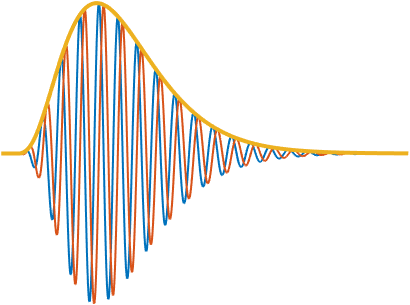
\includegraphics[height=2cm,width=3.5cm]{gammatone_Q8.png}}
 \put(2.5,0.0){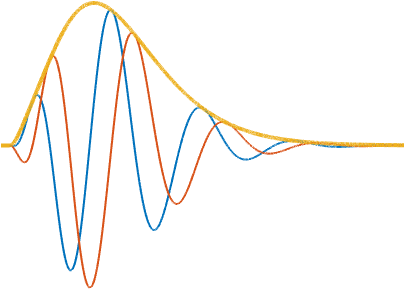
\includegraphics[height=2cm,width=3.5cm]{gammatone_Q1.png}}
\end{picture}
\caption{
\label{fig:gammatones}
Left: Gammatone wavelet $\boldsymbol{\psi_{\gamma_1}}(t)$ with a quality factor of $Q_1=8$.
Right: Gammatone wavelet $\boldsymbol{\psi_{\gamma_2}}(t)$ with a quality factor of $Q_2=1$.}
\end{center}
\end{figure}

Wavelets
$\boldsymbol{\psi_{\gamma_1}}(t)$ and $\boldsymbol{\psi_{\gamma_2}}(t)$ are designed as fourth-order Gammatone
wavelets with one vanishing moment \cite{Venkitaraman2014}, as shown in Figure \ref{fig:gammatones}.
In the context of auditory scene analysis, the asymmetric envelope of Gammatone wavelets is more biologically plausible than the symmetric, Gaussian-like envelope of the widespread Morlet wavelets.
Indeed, it allows to reproduce two important psychoacoustic effects in the mammalian cochlea: the asymmetry of temporal masking and the asymmetry of spectral masking \cite{Fastl2007}.
Moreover, it should be noted that Gammatone wavelets follow the typical amplitude profile of natural sounds, beginning with a relatively sharp attack and ending with a slower decay.

The next subsection extends the second-order scattering operator to joint wavelet transforms over the time and log-frequency variables.

\subsection{Time-frequency scattering}
\cite{Anden2015}

\begin{equation}
\boldsymbol{\psi_{\gamma_{\mathrm{fr}}, \theta_{\mathrm{fr}}}}(\gamma_1)
= \theta_{\mathrm{fr}} 2^{-\gamma_{\mathrm{fr}}/Q_{\mathrm{fr}}}
\boldsymbol{\psi_{\theta_{\mathrm{fr}}}}( \theta_{\mathrm{fr}}  2^{-\gamma_{\mathrm{fr}}/Q_{\mathrm{fr}}}\gamma_1)
\end{equation}

\begin{equation}
\boldsymbol{x_2}(t,\gamma_1,\gamma_2,\gamma_{\mathrm{fr}},\theta_{\mathrm{fr}}) =
\vert \boldsymbol{x_1}
\overset{t}{\ast} \boldsymbol{\psi_{\gamma_2}}
\overset{\gamma_1}{\ast} \boldsymbol{\psi_{\gamma_{\mathrm{fr}}, \theta_{\mathrm{fr}}}}
\vert (t,\gamma_1)
\end{equation}
Again, we use the generic literal $\gamma$ as a shorthand for $\gamma_1$ or $(\gamma_1, \gamma_2, \gamma_{\mathrm{fr}}, \theta_{\mathrm{fr}})$.

\section{Unsupervised approach}

GL

\subsection{Results}

GL

\section{Supervised approach}

\subsection{Results}

VL

\section{Discussion}

ML

\section{Conclusion}

ML

\bibliographystyle{unsrt}
\bibliography{biblio}

% biography section
% 
% If you have an EPS/PDF photo (graphicx package needed) extra braces are
% needed around the contents of the optional argument to biography to prevent
% the LaTeX parser from getting confused when it sees the complicated
% \includegraphics command within an optional argument. (You could create
% your own custom macro containing the \includegraphics command to make things
% simpler here.)
%\begin{IEEEbiography}[{\includegraphics[width=1in,height=1.25in,clip,keepaspectratio]{mshell}}]{Michael Shell}
% or if you just want to reserve a space for a photo:

%\begin{IEEEbiography}{Mathieu Lagrange}
%Biography text here.
%\end{IEEEbiography}

% if you will not have a photo at all:
%\begin{IEEEbiographynophoto}{John Doe}
%Biography text here.
%\end{IEEEbiographynophoto}

% insert where needed to balance the two columns on the last page with
% biographies
%\newpage

%\begin{IEEEbiographynophoto}{Jane Doe}
%Biography text here.
%\end{IEEEbiographynophoto}

% You can push biographies down or up by placing
% a \vfill before or after them. The appropriate
% use of \vfill depends on what kind of text is
% on the last page and whether or not the columns
% are being equalized.

%\vfill

% Can be used to pull up biographies so that the bottom of the last one
% is flush with the other column.
%\enlargethispage{-5in}



% that's all folks
\end{document}


